\documentclass[11pt]{article}

\usepackage[margin=1in]{geometry}
\usepackage{graphicx}
\usepackage{booktabs}
\usepackage{array}
\usepackage{multirow}
\usepackage{xcolor}
\usepackage{hyperref}
\usepackage[numbers,sort&compress]{natbib}
\usepackage{caption}
\usepackage{subcaption}
\usepackage{xurl}
\usepackage{tabularx}

\hypersetup{
  colorlinks=true,
  linkcolor=blue!50!black,
  citecolor=blue!50!black,
  urlcolor=blue!50!black
}

\graphicspath{{../figures/}}

\title{AutoTeaKG-Silver: An Uncertainty-Aware Evidence Graph for Tea Functional Activity Literature}
\author{Anonymous Authors}
\date{}

\begin{document}
\maketitle

\begin{abstract}
Tea, tea extracts, and tea-derived components are widely studied for antioxidant, anti-inflammatory, metabolic, cardiovascular, neuroprotective, and gut-microbiota-related activities. However, the evidence is fragmented across tea types, component definitions, processing conditions, model systems, and endpoint labels, making it difficult to compare claims or identify where evidence is strong. We introduce AutoTeaKG-Silver, an automatically generated, provenance-rich, uncertainty-aware evidence graph for tea functional activity literature. The system retrieves PubMed records, converts title/abstract and open full-text methods sections into structured evidence records, normalizes activity and evidence labels, extracts processing and extraction context, and exports a graph in which every edge retains source provenance and uncertainty attributes. In the current KG v3 release, AutoTeaKG-Silver contains 635 evidence records, 1,989 nodes, and 8,195 edges. The pipeline increases processing-context coverage from 146 to 183 records and extraction-context coverage from 154 to 185 records, while explicitly preserving 303 records whose processing or extraction context remains missing. The resulting resource exposes uneven evidence support across activity classes, identifies processing-context reporting gaps, and provides a microbiome-ready graph substrate for downstream mechanism queries. AutoTeaKG-Silver should therefore be interpreted not as a manually verified gold-standard database, but as a reproducible silver-standard evidence infrastructure for living tea bioactivity synthesis.
\end{abstract}

\noindent\textbf{Database URL:} \url{https://github.com/ShawnXiha/AutoTeaKG_Silver}

\begin{figure}[t]
  \centering
  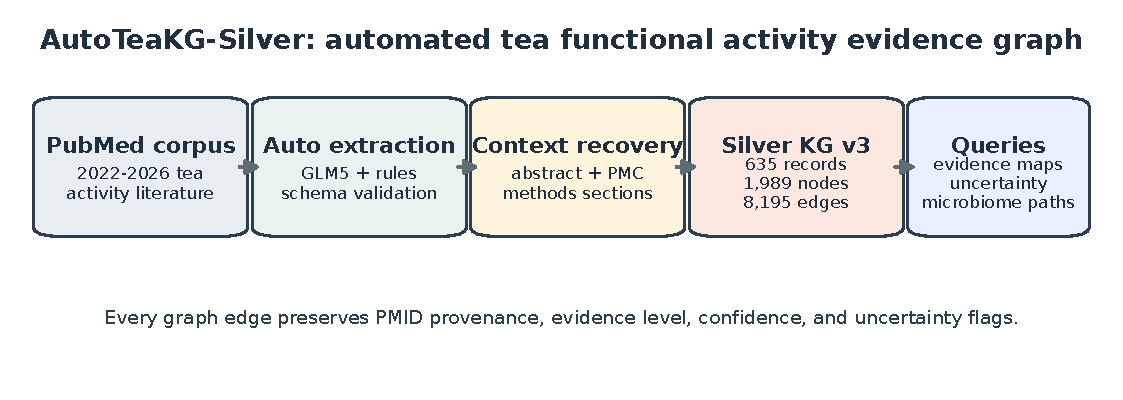
\includegraphics[width=\linewidth]{fig_graphical_abstract.pdf}
  \caption{Graphical overview of AutoTeaKG-Silver. The pipeline converts PubMed tea functional activity literature into structured evidence records, recovers processing and extraction context from abstracts and open PMC methods sections, and exports a provenance-rich uncertainty-aware evidence graph.}
  \label{fig:graphical_abstract}
\end{figure}

\section{Introduction}

Tea is a chemically complex beverage and botanical material with a large literature on potential health-related functions. Reviews have summarized the biological potential of catechins, theaflavins, theanine, caffeine, polysaccharides, and other tea-derived compounds across antioxidant, inflammatory, metabolic, cardiovascular, and neuroprotective endpoints~\cite{luo2024tea_bioactive_review,yang2025bioavailability_tea_polyphenols,rashwan2025tea_polysaccharides_review}. A parallel literature studies how tea processing and extraction alter chemical profiles and product quality~\cite{raghunath2023tea_extraction_review,aaqil2023black_tea_processing_review,wang2024processing_metabolomics}. More recently, tea--microbiome interactions have become a prominent mechanistic theme, especially for metabolic and gut-brain-axis phenotypes~\cite{zhao2024processed_tea_microbiota,song2024oolong_neuroprotection,tian2024obesity_microbiota}. These bodies of work make tea an attractive domain for structured evidence synthesis.

The central difficulty is that tea functional activity evidence is abundant but poorly aligned. A claim about ``green tea'', ``EGCG'', ``tea polyphenols'', ``fermented tea'', or ``tea polysaccharides'' may refer to different materials, processing states, extraction methods, doses, and experimental settings. Evidence strength also varies substantially: animal studies, in vitro experiments, randomized trials, cohort studies, and narrative reviews often appear together in the same prose summary. Narrative reviews are useful for expert interpretation, but they do not provide a machine-readable evidence layer that can answer comparative questions such as which activities have human evidence, which are mostly preclinical, or whether processing information is reported at all.

Existing tea databases do not solve this functional evidence problem. TeaPVs and TeaNekT provide genomic and transcriptomic resources for tea plant biology~\cite{an2022teapvs,zheng2024teanekt}. TRSRD is closer to a tea-domain knowledge graph, but it focuses on risky substances rather than functional activity evidence~\cite{wang2023trsrd}. More general natural-product resources such as NPASS and natural-product drug-interaction knowledge graphs show that natural products can be represented computationally~\cite{zhao2023npass_update,taneja2023npdi_kg}, but they do not encode the tea-specific combination of functional activity, processing context, evidence level, and microbiome mechanism.

We argue that the missing contribution is not another static spreadsheet of tea papers, but an automated evidence infrastructure that makes uncertainty explicit. Manual curation can improve record quality, but it does not scale to a living PubMed-updated resource. Conversely, raw large-language-model extraction is not sufficient unless outputs are constrained by domain schemas, provenance, validation flags, and uncertainty classes. The practical goal is therefore to build a silver-standard graph: a resource that is automatically generated, reproducible, inspectable, and useful for evidence mapping, while avoiding the stronger claim that every edge is expert verified.

This paper introduces AutoTeaKG-Silver, an uncertainty-aware evidence graph for tea functional activity literature. The pipeline retrieves PubMed records, generates structured evidence records, extracts tea type, component group, activity category, study type, evidence level, mechanism labels, microbiome features, and host phenotypes, and then enriches records with processing and extraction context from abstracts and open full-text methods sections. The final graph preserves evidence-record nodes so that each relation can be traced back to a paper, raw claim text, evidence level, and uncertainty flag.

The contributions are fourfold. First, we define a graph-ready evidence model for tea functional activity literature that separates activity claims from study design, evidence level, component context, processing context, and uncertainty. Second, we build an automated silver-standard resource with 635 evidence records and 8,195 graph edges, excluding manual annotation as a data-generation dependency. Third, we show that processing and extraction context remain a measurable bottleneck: targeted extraction improves coverage, but many records lack open full-text or report insufficient methods detail. Fourth, we provide figure-ready query tables and graph outputs that support evidence mapping, processing-aware analysis, and microbiome mechanism exploration.

\subsection{Prior work and resource gap}

\subsubsection{Tea bioactivity reviews and evidence synthesis}

The tea bioactivity literature is rich in narrative synthesis. Recent reviews summarize the biological potential of tea bioactive compounds across inflammation, oxidation, metabolism, microbiota modulation, and other health-related endpoints~\cite{luo2024tea_bioactive_review}. Other reviews focus on specific mechanistic constraints, such as the bioavailability of tea polyphenols and the difficulty of extrapolating in vitro activity to in vivo health effects~\cite{yang2025bioavailability_tea_polyphenols}. Tea polysaccharides have also become a distinct review topic because their chemical characterization, conjugates, and bioactivities differ from those of catechin-centered polyphenol literature~\cite{rashwan2025tea_polysaccharides_review}. These reviews establish that the domain is active and biologically broad, but their outputs remain prose summaries rather than computable evidence records. AutoTeaKG-Silver differs by representing study type, evidence level, activity category, component context, and uncertainty as queryable fields.

\subsubsection{Processing-aware tea chemistry and microbiome mechanisms}

Tea processing and extraction strongly influence chemical composition, product quality, and downstream interpretation. Food engineering reviews describe ultrasound, microwave, pressurized-liquid, supercritical, and other extraction technologies for recovering tea bioactives~\cite{raghunath2023tea_extraction_review}. Tea processing reviews further show that harvesting, withering, rolling, fermentation or oxidation, drying, and storage can alter phytochemical profiles, especially in black tea and fermented products~\cite{aaqil2023black_tea_processing_review}. Metabolomics studies provide analytical evidence that processing technology changes tea quality and chemical profiles~\cite{wang2024processing_metabolomics}. In parallel, microbiome-focused work links differently processed tea, tea polyphenols, fermented tea, and tea polysaccharides to gut microbiota, microbial metabolites, host barrier function, metabolic outcomes, and cognition-related phenotypes~\cite{zhao2024processed_tea_microbiota,song2024oolong_neuroprotection,tian2024obesity_microbiota,zhang2024fermented_tea_microbiota,arce2025kombucha_rct}. These studies motivate the processing-aware and microbiome-aware dimensions of AutoTeaKG-Silver.

\subsubsection{Tea databases, natural-product resources, and knowledge graphs}

Existing tea resources address important but different layers of tea biology. TeaPVs focuses on genomic variation in \textit{Camellia sinensis}, and TeaNekT provides comparative transcriptomic information for tea plant biology~\cite{an2022teapvs,zheng2024teanekt}. TRSRD uses natural-language processing and knowledge graph techniques for tea risky-substance research, but the target domain is risk and safety rather than functional activity evidence~\cite{wang2023trsrd}. Broader natural-product resources such as NPASS provide quantitative activity and species-source information, and natural-product drug-interaction knowledge graphs show the feasibility of graph-based representation for natural products~\cite{zhao2023npass_update,taneja2023npdi_kg}. AutoTeaKG-Silver is complementary to these resources: it targets tea functional activity claims, evidence strength, processing/extraction context, microbiome mechanisms, and uncertainty-aware provenance.

\section{Materials and Methods}

\subsection{Corpus construction and retrieval archive}

The corpus was constructed from PubMed searches over tea functional activity, component, processing, extraction, microbiome, and human-evidence query blocks. The archived query set covered the publication window from 2022-01-01 to 2026-03-31 and included broad review retrieval, functional activity primary studies, microbiome-focused studies, processing-aware studies, and human evidence searches. Across the larger retrieval batches, records were deduplicated by PMID and normalized into paper-level metadata tables. The manuscript uses the locked auto-only evidence graph derived from these retrievals rather than manually adjudicated mini-gold records.

\subsection{Evidence-record schema}

Each evidence record represents a structured claim anchored to a source paper. Core fields include the source paper identifier, tea type, material form, component group, activity category, endpoint label, study type, evidence level, model system, dose or exposure text, effect direction, mechanism label, microbiota taxon, microbial metabolite, host phenotype, raw claim text, confidence score, and provenance metadata. Activity categories include antioxidant, anti-inflammatory, metabolic improvement, anti-obesity, gut microbiota modulation, neuroprotection, cardiovascular protection, and other. Evidence levels distinguish preclinical in vivo evidence, human observational evidence, human interventional evidence, evidence synthesis, non-quantitative evidence synthesis, and low-preclinical evidence.

\subsection{Auto-only extraction pipeline}

AutoTeaKG-Silver was designed as an auto-only pipeline. The construction path used PubMed metadata, title/abstract text, candidate-record heuristics, GLM5 title/abstract extraction, schema validation, post-processing, duplicate consolidation, and graph export. Manual audit worksheets, mini-gold annotations, and adjudication logs were excluded from the data-generation path. This design choice is deliberate: the goal is to create a scalable silver-standard evidence layer whose uncertainty is visible, rather than to claim expert-level verification for each relation.

\begin{table}[t]
\centering
\small
\caption{Compact construction-stage summary. Detailed scripts and output paths are listed in Appendix~\ref{app:reproducibility}.}
\label{tab:pipeline_stages}
\begin{tabular}{p{0.34\linewidth}p{0.28\linewidth}p{0.25\linewidth}}
\toprule
Stage & Output & Count or result \\
\midrule
PubMed retrieval and normalization & archived query batches & 5 query blocks \\
Auto-only evidence extraction & silver evidence records & 635 records \\
Abstract-level context recovery & processing/extraction patches & 365 patches \\
PMC methods retrieval & methods-like sections & 151 records \\
Methods-level context recovery & methods-section patches & 151 patches \\
Vocabulary-normalized KG v3 & graph and figure tables & 1,989 nodes; 8,195 edges \\
\bottomrule
\end{tabular}
\end{table}

\subsection{Processing and extraction context recovery}

Processing and extraction context were recovered in three stages. The first stage used conservative rule-based matching over titles, abstracts, and claim text. The second stage targeted records flagged as missing processing or extraction context and prompted GLM5 to extract only tea-material processing, extraction, and component context from title/abstract text. The third stage queried NCBI E-utilities to map PMIDs to open PMC full text, extracted methods-like sections, and ran a targeted methods-section extractor on records with available full-text context. All targeted extraction steps were patch-first: the model generated a patch table, and patched copies of the silver dataset and KG were regenerated rather than overwriting the base resource.

\subsection{Vocabulary normalization}

LLM surface labels were normalized into a controlled processing and extraction vocabulary. For example, black tea manufacturing and black tea formation were mapped to black tea processing; brick-like form and brick tea processing were mapped to compressed/brick tea processing; cold brewing and hot brewing were mapped to brewing/infusion; and isolation, isolated, and purification were mapped to isolation/purification. Raw LLM labels were retained in mapping tables so that normalization decisions remain auditable.

\subsection{Uncertainty assignment}

Each record was assigned uncertainty flags and an uncertainty class. Flags captured low LLM confidence, missing processing or extraction context, generic mechanism labels, missing named microbiota, taxonomy expansion needs, preclinical-only evidence, review-summary records, uncertain effect direction, and schema validation problems. The uncertainty class summarized these signals into low, moderate, or high uncertainty. This design keeps uncertainty in the graph rather than hiding it during filtering.

\paragraph{Uncertainty model.}
AutoTeaKG-Silver assigns uncertainty at the evidence-record level and propagates the same uncertainty attributes to graph edges through the evidence-record node. The silver confidence score combines the original extraction confidence with record specificity and context completeness. Context completeness assigns partial credit for non-generic tea type, component group, processing step, and extraction method. Mechanism specificity distinguishes missing or generic mechanisms from pathway-like or named mechanism labels. Records are then assigned uncertainty flags (Appendix Table~\ref{tab:uncertainty_flags}) and mapped to low, moderate, or high uncertainty classes using the rules in Table~\ref{tab:uncertainty_classes}.

\begin{table}[t]
\centering
\small
\caption{Uncertainty-class assignment rules. The severe flag set includes low LLM confidence, taxonomy expansion needed, missing component context, generic mechanism, and invalid controlled-vocabulary labels.}
\label{tab:uncertainty_classes}
\begin{tabular}{p{0.26\linewidth}p{0.55\linewidth}p{0.12\linewidth}}
\toprule
Class & Rule & Final count \\
\midrule
Low uncertainty & Silver confidence $\geq 0.80$ and no severe uncertainty flag. & 100 \\
Moderate uncertainty & Silver confidence $\geq 0.60$ and at most two severe uncertainty flags. & 470 \\
High uncertainty & All remaining records. & 65 \\
\bottomrule
\end{tabular}
\end{table}

\subsection{Graph construction and query tables}

The graph preserves papers and evidence records as explicit nodes. Evidence records are linked to tea type, material form, component group, processing step, extraction method, activity category, study type, evidence level, effect direction, mechanisms, microbiota features, metabolites, host phenotypes, and uncertainty flags. Graph edges retain paper identifier, record identifier, evidence level, study type, effect direction, confidence score, and uncertainty class. Query tables were generated from the final KG v3 to support evidence mapping, activity-by-evidence heatmaps, uncertainty summaries, processing and extraction label distributions, microbiome mechanism subsets, and node/edge composition summaries.

\subsection{External validation protocol}

To avoid using manual review as a hidden construction dependency, validation is separated from graph generation. We prepared a stratified validation sample of 48 auto-only evidence records: 14 low-uncertainty records, 24 moderate-uncertainty records, and 10 high-uncertainty records. The validation worksheet asks reviewers to assess activity category, study type, evidence level, component group, processing step, extraction method, and mechanism label as correct, minor issue, major issue, or not applicable. Overall record decisions are recorded as accept, accept with correction, or reject. The validation files are released with the manuscript package, but the current KG v3 is not trained on or modified by this validation sample.

\subsection{Reproducibility package}

The current manuscript release is organized so that each result can be traced to a script and output directory (Table~\ref{tab:pipeline_stages}). The final graph used for all Results figures is the vocabulary-normalized methods-level KG v3. The corresponding record table, node table, edge table, query tables, and figure-generation script are listed in Appendix~\ref{app:reproducibility}.

\section{Results}

\subsection{AutoTeaKG-Silver constructs a provenance-rich tea functional activity graph}

The final KG v3 contains 635 silver evidence records, 1,989 nodes, and 8,195 edges (Figure~\ref{fig:kg_composition}). The graph includes paper nodes, evidence-record nodes, activity-category nodes, study-type nodes, evidence-level nodes, tea and component context nodes, processing and extraction context nodes, mechanism nodes, microbiota-feature nodes, microbial-metabolite nodes, host-phenotype nodes, and uncertainty-flag nodes. The explicit EvidenceRecord layer is important because it prevents mechanistic and activity relations from becoming detached from their source papers.

\begin{table}[t]
\centering
\small
\caption{Final KG v3 summary statistics used throughout the Results section.}
\label{tab:dataset_stats}
\begin{tabular}{lr}
\toprule
Quantity & Count \\
\midrule
Silver evidence records & 635 \\
KG nodes & 1,989 \\
KG edges & 8,195 \\
Microbiome-relevant records & 190 \\
Records with processing context & 183 \\
Records with extraction context & 185 \\
Low-uncertainty records & 100 \\
Moderate-uncertainty records & 470 \\
High-uncertainty records & 65 \\
Residual missing-context records & 303 \\
\bottomrule
\end{tabular}
\end{table}

\begin{figure}[t]
  \centering
  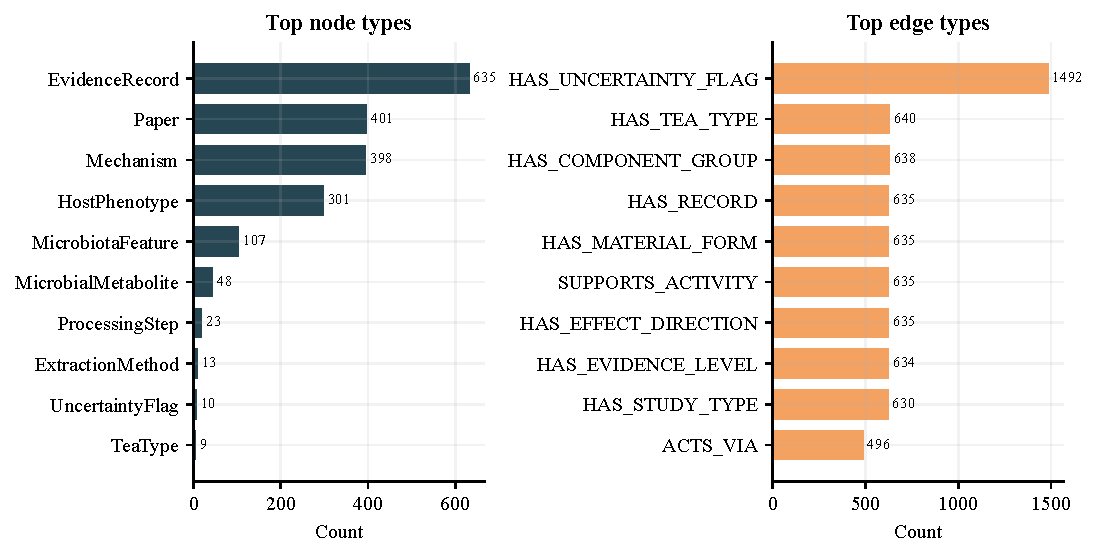
\includegraphics[width=\linewidth]{fig_kg_composition.pdf}
  \caption{Node and edge type composition of KG v3. The graph preserves evidence-record provenance while linking papers, activity categories, evidence levels, tea/component context, processing/extraction context, mechanisms, microbiota features, metabolites, phenotypes, and uncertainty flags.}
  \label{fig:kg_composition}
\end{figure}

\subsection{Evidence-level normalization exposes uneven support across activity classes}

The activity-by-evidence heatmap shows that tea functional activity claims are not evenly supported across evidence levels (Figure~\ref{fig:activity_evidence}). Several activity categories are dominated by preclinical in vivo records and non-quantitative evidence syntheses, while human observational and interventional evidence is concentrated in fewer categories. This pattern supports the central motivation for evidence grading: without evidence-level normalization, review-derived, animal, cohort, and randomized-trial claims are easily mixed into a single apparent evidence base.

\begin{figure}[t]
  \centering
  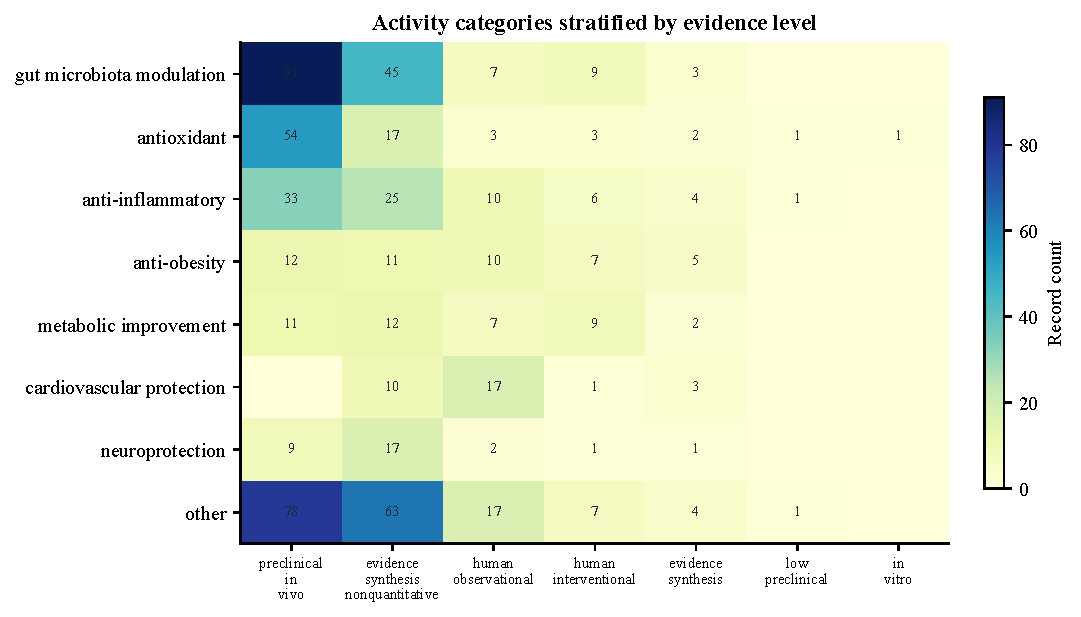
\includegraphics[width=\linewidth]{fig_activity_evidence_heatmap.pdf}
  \caption{Heatmap of normalized activity categories stratified by evidence level in KG v3. The distribution shows that animal evidence and non-quantitative evidence syntheses dominate several activity categories, while human interventional and observational evidence is concentrated in fewer endpoints.}
  \label{fig:activity_evidence}
\end{figure}

\subsection{Targeted extraction improves but does not eliminate missing processing context}

Processing and extraction context increased across extraction stages (Figure~\ref{fig:context_coverage}). Rule-based extraction identified processing context in 146 records and extraction context in 154 records. Abstract-level targeted GLM5 extraction increased coverage, and PMC methods-section extraction further raised processing-context coverage to 183 records and extraction-context coverage to 185 records. The improvement is measurable but modest, indicating that processing context is not uniformly available from abstracts alone.

\begin{table}[t]
\centering
\small
\caption{Stage-wise ablation and quality-control summary. Each stage adds context or normalizes previous outputs while preserving a zero unresolved-edge graph export. Proc., processing-context records; Extr., extraction-context records; Missing, records still flagged for missing processing or extraction context.}
\label{tab:stagewise_qc}
\begin{tabular}{p{0.32\linewidth}rrrrrr}
\toprule
Stage & Proc. & Extr. & Missing & Unmapped & Errors & Bad edges \\
\midrule
Rules-only silver layer & 146 & 154 & 365 & -- & -- & 0 \\
Abstract-level targeted LLM & 167 & 170 & 329 & 0 & 0 & 0 \\
Methods-section targeted LLM & 183 & 185 & 303 & 0 & 0 & 0 \\
\bottomrule
\end{tabular}
\end{table}

The stage-wise quality-control summary shows that each pipeline stage contributes measurable context recovery while preserving graph integrity (Table~\ref{tab:stagewise_qc}). Processing-context coverage increased from 146 records in the rules-only silver layer to 167 records after abstract-level targeted extraction and 183 records after methods-section extraction. Extraction-context coverage increased from 154 to 170 and then to 185 records. The missing-context flag decreased from 365 to 303 records, while the final normalized KG retained zero unmapped processing/extraction labels and zero unresolved graph edges.

\begin{figure}[t]
  \centering
  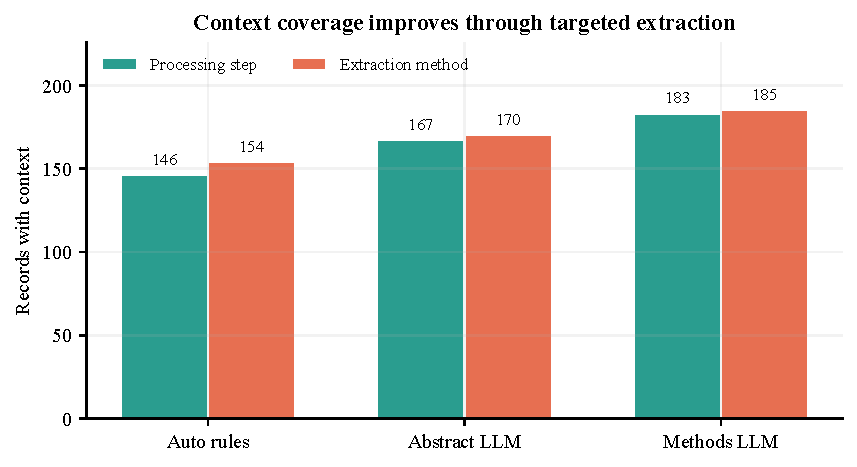
\includegraphics[width=.82\linewidth]{fig_context_coverage.pdf}
  \caption{Context recovery across automated extraction stages. Rule-based extraction established the initial context layer, abstract-level targeted GLM5 extraction added additional context, and PMC methods-section extraction further improved recovery of processing and extraction variables.}
  \label{fig:context_coverage}
\end{figure}

The full-text retrieval analysis clarified why context remains missing. Of 329 records still flagged after abstract-level extraction, 151 records had PMC methods-like sections, while 178 lacked open PMC full text (Figure~\ref{fig:fulltext_funnel}). Methods-section extraction generated patches for all 151 available records and recovered details such as crushing and sieving, cleaning--drying--powdering, steaming and fixation, ultrasonic ethanol extraction, methanol sonication, microwave-assisted extraction, brewing, and isolation/purification.

\begin{figure}[t]
  \centering
  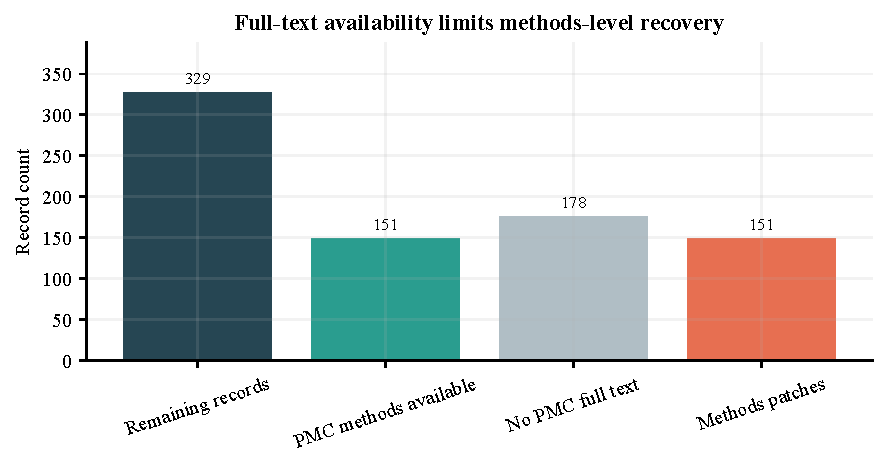
\includegraphics[width=.82\linewidth]{fig_fulltext_methods_funnel.pdf}
  \caption{Full-text methods availability funnel for records that remained missing context after abstract-level extraction. Of 329 remaining records, PMC methods-like sections were available for 151 records, while 178 records lacked open PMC full text.}
  \label{fig:fulltext_funnel}
\end{figure}

\subsection{Vocabulary normalization reduces processing and extraction label fragmentation}

Processing and extraction labels generated by LLM extraction required normalization before graph use. The final vocabulary-normalized KG reduced surface-form fragmentation while retaining raw labels for provenance. Fermentation/oxidation was the dominant processing context, followed by storage/aging, enzymatic treatment, roasting, black tea processing, processing category contrast, drying, steaming/fixation, and crushing/grinding/sieving. Extraction labels were concentrated in other extraction, aqueous extraction, isolation/purification, analytical characterization, brewing/infusion, solvent extraction, ultrasound-assisted extraction, and commercial preparation (Figure~\ref{fig:processing_labels}).

\begin{figure}[t]
  \centering
  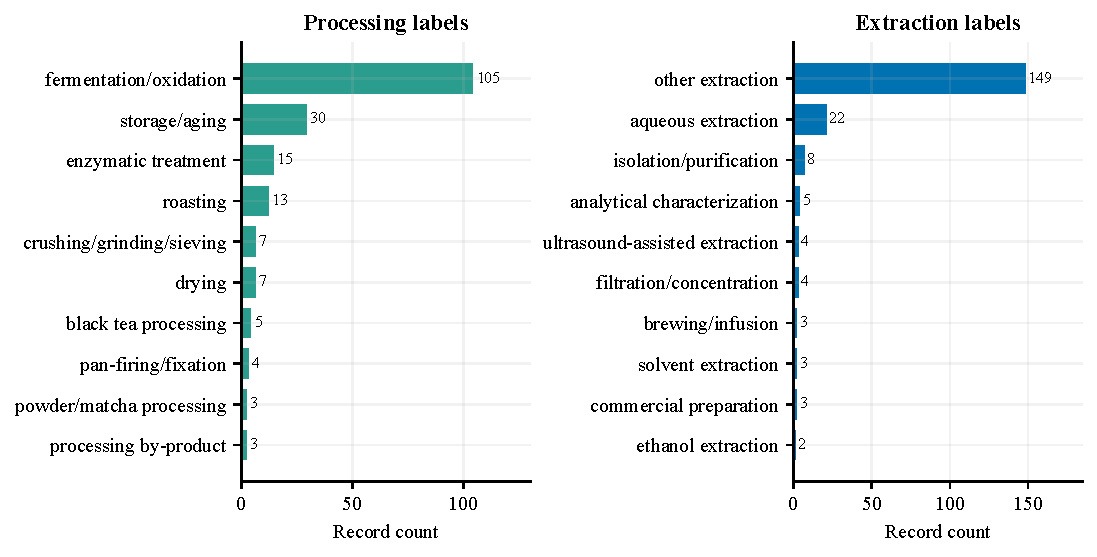
\includegraphics[width=\linewidth]{fig_processing_extraction_labels.pdf}
  \caption{Top normalized processing and extraction labels after abstract-level and methods-section extraction. Vocabulary normalization reduces LLM label fragmentation by mapping surface forms such as black tea manufacturing, matcha production, brewing, isolation, and chromatographic analysis into controlled context labels.}
  \label{fig:processing_labels}
\end{figure}

\subsection{Uncertainty classes make silver-standard status explicit}

The final KG contains 100 low-uncertainty records, 470 moderate-uncertainty records, and 65 high-uncertainty records. The activity-level uncertainty composition (Figure~\ref{fig:uncertainty}) shows that moderate uncertainty dominates the resource. This result is not a defect of the resource; it is the intended operating mode of a silver-standard evidence graph. Instead of filtering uncertainty away, AutoTeaKG-Silver stores uncertainty as a queryable property that downstream users can use to restrict analyses.

\begin{figure}[t]
  \centering
  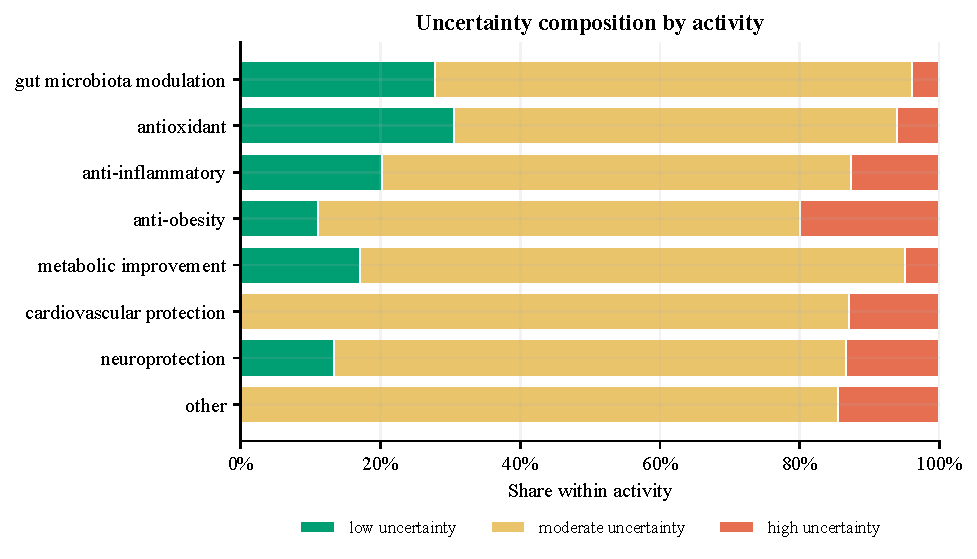
\includegraphics[width=\linewidth]{fig_uncertainty_by_activity.pdf}
  \caption{Uncertainty composition by activity category. Each record was assigned an uncertainty class based on LLM confidence, schema validity, mechanism specificity, context completeness, evidence level, and taxonomy status.}
  \label{fig:uncertainty}
\end{figure}

\subsection{The graph supports microbiome-mechanism queries}

KG v3 contains 190 microbiome-relevant records. These records connect tea types and component groups to gut microbiota modulation, microbial metabolites, host phenotypes, and mechanism labels. The microbiome subset provides a graph-native substrate for querying component--microbiota--metabolite--phenotype paths rather than treating microbiome mentions as isolated keywords. This design is motivated by recent work linking tea polyphenols, oolong tea polyphenols, and tea polysaccharides to microbiota-mediated metabolic, inflammatory, and neuroprotective programs~\cite{zhao2024processed_tea_microbiota,song2024oolong_neuroprotection,tian2024obesity_microbiota,zhang2024fermented_tea_microbiota,arce2025kombucha_rct}.

\subsection{A graph query recovers a tea-polysaccharide gut-liver axis pattern}

To test whether the KG supports structured queries beyond flat keyword retrieval, we queried records with tea-polysaccharide component context and microbiome/metabolite/host-phenotype fields. The query recovered five representative records linking tea polysaccharides to gut microbiota modulation, butyric acid or SCFA-related metabolites, and liver, barrier, or lipid-deposition phenotypes (Table~\ref{tab:graph_query_case}; Figure~\ref{fig:graph_query_case}). The retrieved paths preserve evidence level and uncertainty class, allowing the user to distinguish low-uncertainty preclinical gut-liver-axis records from broader moderate-uncertainty microbiome records. This query illustrates the practical advantage of the graph representation: component, microbiome, metabolite, phenotype, evidence, and uncertainty constraints can be applied together rather than searched as independent keywords.

\begin{table}[t]
\centering
\small
\caption{Graph query case study for tea-polysaccharide microbiome mechanisms. The query selects records with tea-polysaccharide component context and microbiome/metabolite/host-phenotype evidence.}
\label{tab:graph_query_case}
\begin{tabularx}{\linewidth}{p{0.12\linewidth}p{0.18\linewidth}Xp{0.22\linewidth}p{0.11\linewidth}}
\toprule
Record & Tea/component & Mechanism or path & Metabolite / phenotype & Evidence \\
\midrule
41899489-R1 & black tea; polysaccharides & gut-liver axis; macrophage M2 shift & butyric acid; reduced liver inflammation & preclinical; low \\
41899489-R2 & black tea; polysaccharides & microbiota production of butyric acid & butyric acid & preclinical; low \\
41475763-R1 & tea; polysaccharides & enrichment of SCFA producers & butyrate, acetate, propionate; reduced hepatic lipid deposition & preclinical; moderate \\
41475763-R2 & tea; polysaccharides & microbiota-gut-liver axis signaling & butyrate, isovalerate; reduced LDL-C and hepatic lipid deposition & preclinical; moderate \\
41861686-R1 & yellow tea; polysaccharides & barrier-related mechanism & SCFAs; intestinal barrier integrity & preclinical; low \\
\bottomrule
\end{tabularx}
\end{table}

\begin{figure}[t]
  \centering
  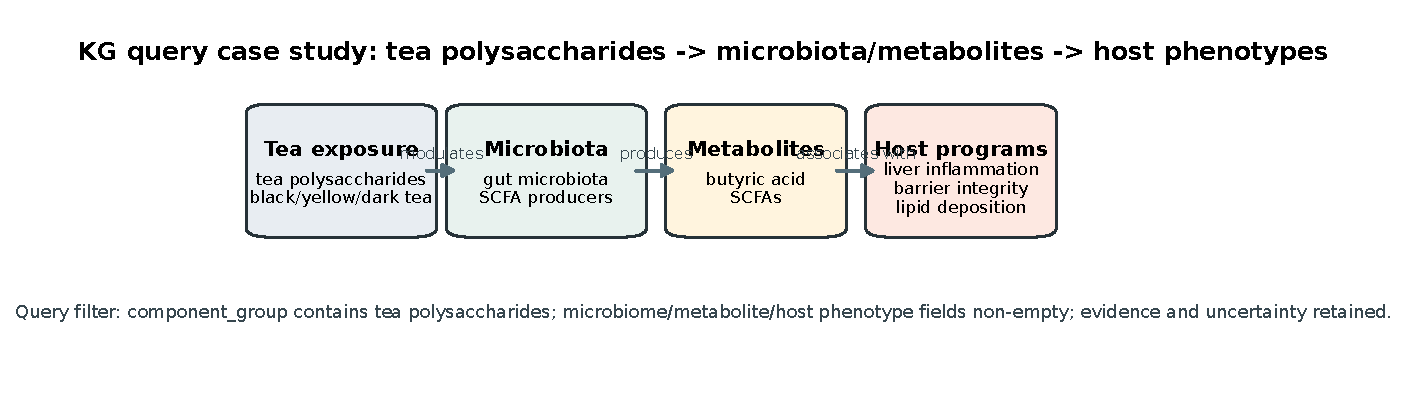
\includegraphics[width=.92\linewidth]{fig_graph_query_polysaccharide_microbiome.pdf}
  \caption{Graph query case study linking tea polysaccharides to microbiota/metabolite and host-phenotype nodes. The query keeps evidence level and uncertainty class attached to each evidence record.}
  \label{fig:graph_query_case}
\end{figure}

\section{Discussion}

AutoTeaKG-Silver reframes tea functional activity synthesis as an automated evidence-graph construction problem. The main contribution is not that the system replaces expert review. Rather, the system creates a reproducible and updateable substrate that makes evidence level, provenance, missing context, and uncertainty visible. This framing is important because tea bioactivity claims often differ in study design, material identity, processing state, and mechanism specificity.

The results show that evidence grading changes interpretation. Tea functional activity categories contain a mixture of animal studies, human studies, meta-analyses, randomized trials, and reviews. Treating these records as equivalent would inflate confidence in claims that remain mostly preclinical. By encoding evidence level and study type as first-class graph attributes, AutoTeaKG-Silver allows users to query the evidence base under stricter assumptions.

The processing-context experiments reveal a second challenge. Processing and extraction variables are essential for interpreting tea chemistry and activity, yet many abstracts omit these details. Targeted LLM extraction and PMC methods retrieval improve coverage, but 303 records remain flagged for missing processing or extraction context. This result suggests that future improvements should focus on full-text access and methods-section extraction rather than repeatedly prompting abstracts.

The uncertainty layer is a practical compromise between scale and reliability. A manually curated gold-standard resource would be smaller and slower to update. A raw LLM graph would be larger but difficult to trust. AutoTeaKG-Silver occupies the middle ground: it keeps all records provenance-rich, marks uncertainty explicitly, and provides query tables and figures that can be regenerated from the graph.

\section{Limitations}

This work has four important limitations. First, AutoTeaKG-Silver is a silver-standard resource, not a manually verified gold-standard database. The graph should be used with uncertainty filters when precise biological conclusions are required. Second, the current system relies on PubMed abstracts and open PMC full text; records without PMC full text remain difficult to refine. Third, processing and extraction labels are normalized by rules after LLM extraction, but some labels still represent broad process categories rather than complete experimental protocols. Fourth, the microbiome subgraph includes grouped taxa and generic mechanism labels, so causal interpretation requires additional normalization and full-text validation.

\section{Conclusion}

AutoTeaKG-Silver demonstrates that tea functional activity literature can be converted into an automated, provenance-rich, uncertainty-aware evidence graph. The current KG v3 release contains 635 evidence records, 1,989 nodes, and 8,195 edges, and provides figure-ready query tables for evidence mapping, processing-aware analysis, uncertainty assessment, and microbiome mechanism exploration. The results support a practical conclusion: automated evidence graphs can accelerate tea bioactivity synthesis, provided that uncertainty, provenance, and missing context are treated as first-class data rather than hidden errors.

\section*{Data and Code Availability}

All data products, scripts, figure-ready tables, manuscript drafts, and reproducibility artifacts used in this study are organized in the project repository. The current public repository is hosted at \url{git@github.com:ShawnXiha/AutoTeaKG_Silver.git}. The final KG v3 used in the manuscript is stored under \path{reports/methods_processing_vocab_normalized}; the main evidence table is \path{autoteakg_silver_records.csv}, and the graph export is provided as \path{kg_v3/nodes.csv} and \path{kg_v3/edges.csv}. Figure-ready query tables are available under \path{reports/kg_v3_query_tables}. SQLite database files, virtual environments, raw LLM/API response logs, and local cache files are excluded from the public repository because they are either reproducible intermediate artifacts, environment-specific files, or large raw API traces. The processed evidence tables and graph exports are included for reproducibility.

\section*{LLM Usage Statement}

This study used NVIDIA-hosted GLM5 through an OpenAI-compatible API for automatic title/abstract evidence extraction and targeted processing/extraction context recovery. LLM outputs were constrained by schema prompts, post-processed with controlled vocabularies, stored as patch files before merging, and assigned uncertainty flags. LLM extraction was not treated as manual validation. Raw LLM response logs are not included in the public repository; processed patch tables, normalized evidence records, and uncertainty metadata are included. API keys were provided only through environment variables during execution and are not stored in the repository.

\section*{Ethics Statement}

This study analyzes public scientific literature, PubMed metadata, and open PMC full-text sections. It does not involve direct human-subject research, animal experimentation, clinical intervention, or access to private participant-level data. Therefore, institutional review board approval, informed consent, and animal ethics approval are not applicable.

\appendix

\section{Supplementary Data: Reproducibility Paths}
\label{app:reproducibility}

The main manuscript uses the following local release artifacts. Paths are reported relative to the project root.

\begin{table}[htbp]
\centering
\footnotesize
\caption{Key reproducibility artifacts for the current manuscript release.}
\label{tab:repro_paths}
\begin{tabularx}{\linewidth}{p{0.30\linewidth}X}
\toprule
Role & Relative path \\
\midrule
Final KG v3 directory & \path{reports/methods_processing_vocab_normalized} \\
Final silver record table & \path{reports/methods_processing_vocab_normalized/autoteakg_silver_records.csv} \\
Final KG node table & \path{reports/methods_processing_vocab_normalized/kg_v3/nodes.csv} \\
Final KG edge table & \path{reports/methods_processing_vocab_normalized/kg_v3/edges.csv} \\
Figure-ready query tables & \path{reports/kg_v3_query_tables} \\
PubMed search archive & \path{reports/pubmed_search_archive_2026-04-02.md} \\
Silver KG construction & \path{scripts/build_autoteakg_silver_v1.py} \\
Targeted processing extraction & \path{scripts/targeted_processing_llm_extractor.py} \\
PMC methods retrieval & \path{scripts/retrieve_pmc_methods_for_remaining_context.py} \\
Methods extraction batches & \path{scripts/run_methods_processing_extraction_batches.py} \\
Vocabulary normalization & \path{scripts/normalize_processing_extraction_vocab.py} \\
Figure and table generation & \path{scripts/generate_kg_v3_query_tables_and_figures.py} \\
\bottomrule
\end{tabularx}
\end{table}

\section{Supplementary Data: Uncertainty Flag Definitions}
\label{app:uncertainty_flags}

\begin{table}[htbp]
\centering
\scriptsize
\caption{Uncertainty flags used in AutoTeaKG-Silver. Flags are stored on evidence records and propagated to graph edges through the evidence-record node.}
\label{tab:uncertainty_flags}
\begin{tabularx}{\linewidth}{p{0.22\linewidth}p{0.30\linewidth}Xp{0.07\linewidth}}
\toprule
Flag & Trigger & Interpretation & Severity \\
\midrule
\path{low_llm_confidence} & Original LLM confidence score is below 0.80. & The extracted evidence record should be prioritized for review. & severe \\
\path{taxonomy_expansion_needed} & The normalized activity category is \texttt{other}. & The record is either out of scope or requires activity-taxonomy expansion. & severe \\
\path{missing_component_context} & No component group is available after rule and LLM context extraction. & The record lacks a key exposure descriptor. & severe \\
\path{missing_processing_or_extraction_context} & Both processing step and extraction method are empty. & The record cannot support processing-aware comparison. & moderate \\
\path{generic_mechanism} & Mechanism label is empty or belongs to a generic placeholder list. & The record supports an activity claim but weakly supports mechanistic graph reasoning. & severe \\
\path{missing_named_microbiota} & Activity is gut microbiota modulation but no named taxon is extracted. & Microbiome interpretation should remain generic. & moderate \\
\path{preclinical_only} & Study type is animal study. & The claim should not be interpreted as direct human evidence. & moderate \\
\path{review_summary_record} & Study type is systematic review. & The record summarizes literature rather than representing one primary experiment. & moderate \\
\path{low_evidence_level} & Evidence level is low preclinical or in vitro. & The claim has weak translational support. & moderate \\
\path{uncertain_effect_direction} & Effect direction is unclear, no clear effect, or mixed. & The extracted claim should not be counted as straightforward positive support. & moderate \\
\path{missing_abstract} & No abstract text is available. & The record has reduced text evidence for automatic extraction. & moderate \\
\path{invalid_*} & A controlled-vocabulary field contains an invalid label. & The record violates schema constraints and requires normalization or exclusion. & severe \\
\bottomrule
\end{tabularx}
\end{table}

\section{Supplementary Data: Validation Sample}
\label{app:validation}

\begin{table}[htbp]
\centering
\small
\caption{External validation sample design. The sample is stratified by uncertainty class and is released as a worksheet for field-level review. Validation is not used to construct KG v3.}
\label{tab:validation_sample}
\begin{tabular}{lrr}
\toprule
Uncertainty class & Sampled records & Fields reviewed \\
\midrule
Low uncertainty & 14 & 7 \\
Moderate uncertainty & 24 & 7 \\
High uncertainty & 10 & 7 \\
\midrule
Total & 48 & 7 \\
\bottomrule
\end{tabular}
\end{table}

The released worksheet evaluates activity category, study type, evidence level, component group, processing step, extraction method, and mechanism label. Field-level results should be reported only after the worksheet is completed by reviewers.

\bibliographystyle{unsrtnat}
\bibliography{../references/references}

\end{document}
